\documentclass[12pt]{article}

\usepackage{geometry}
 \geometry{
 a4paper,
 left=20mm,
 right=20mm,
 top=20mm,
 bottom=20mm,
 }
\usepackage{polyglossia}
\setmainlanguage{russian} 
\setotherlanguage{english}
\setmainfont{FreeSerif}
\setsansfont{FreeSans}
\setmonofont{FreeMono}

\usepackage{sectsty}

\sectionfont{\fontsize{14}{15}\selectfont}

\usepackage{graphicx} 
\graphicspath{{images/}}
\usepackage{subcaption}

\usepackage{amsmath,bm}

\usepackage{tikz}
\usepackage{float}

\usepackage{svg}

\newcommand*\circled[1]{\tikz[baseline=(char.base)]{
            \node[shape=circle,draw,inner sep=2pt] (char) {#1};}}

\title{Задача № 8 \\ 
Нахождение наименьшего покрытия простого графа}
\author{Гига Максим М8О-113Б-23}
\date{2024}
\begin{document}
\maketitle

\section{Теоретические сведения. Описание алгоритма}

Простым графом называют такой граф $G = (X \cup Y, \Gamma)$, что
\begin{enumerate}
    \item $X \cap Y = \emptyset$
    \item $(\forall X_i \in X) \Gamma X_i \subset Y$
          или $\Gamma^{-1} X_i = \emptyset$
    \item $(\forall Y_j \in Y) \Gamma Y_j = \emptyset$
\end{enumerate}

Простой граф будем обозначать $G = (X, Y, \Gamma)$

Простой граф можно определить также как многозначное
отображение $\Gamma$ конечного множества $X$ в конечное
множество $Y$

Покрытием простого графа $G = (X, Y, \Gamma) = (X, Y, U)$ называют
такое подмножество дуг $W \subset U$, что любая вершина графа
инцидентна по крайней мере одной дуге из $W$

Для того, чтобы простой граф обладал покрытием необходимо и достаточно
выполнение условий:
\begin{enumerate}
    \item $(\forall X_i \in X) \Gamma X_i \ne \emptyset$
    \item $(\forall Y_j \in Y) \Gamma^{-1} Y_j \ne \emptyset$
\end{enumerate}

Минимальное покрытие $W_0$ – это покрытие с минимальным $|W_0|$
то есть с наименьшим числом дуг.

\section{Описание алгоритма, использующего булево
  матричное представление}

Опишем алгоритм позволяющий получить минимальное покрытие
простого графа \\ $G = (X, Y, \Gamma)$, представленного
в виде булевой матрицы $||M||$ размера $m \times n$

\begin{enumerate}
    \item Сопоставим каждой строке $X_i$ матрицы $||M||$
          число $F_i$, равное сумме ее элементов,
          и каждому столоцу $Y_j$ – число $G_j$, равное сумме
          его элементов
    \item Если $\sum F_i = \sum G_j = max(m, n)$ то
          множество дуг, соответствующих единицам,
          дает минимальное покрытие. Если
          $\sum F_i = \sum G_j > max(m, n)$
          то заменяем последовательно
          в произвольном порядке $0$ каждую из единиц
          (условливаясь при этом писать $\circled{1}$ вместо $0$),
          для которой $F_i > 1$ и $G_j > 1$.
    \item В каждой строке с $F_i > 1$ ищем такую
          $1$, что в её столбце найдется
          такая $\circled{1}$, что в строке,
          содержащей эту $\circled{1}$, есть неотмеченная $1$
          с $G_j > 1$. Если $G_j > 1$, то найденная $\circled{1}$
          заменяется на $1$, а найденные $1$ заменяются на
          $\circled{1}$. $F_i$ и $G_j$ обновляются.
          Если, действуя по этому алгоритму,
          невозможно увеличить число $\circled{1}$,
          то $1$ дают минимальное покрытие.
\end{enumerate}

\section{Логическая блок-схема алгоритма}

Основные этапы работы алгоритма представлены на
Рис. \ref*{fig:block_diagram} логической блок
схемы.

\begin{figure}[H]
    \centering
    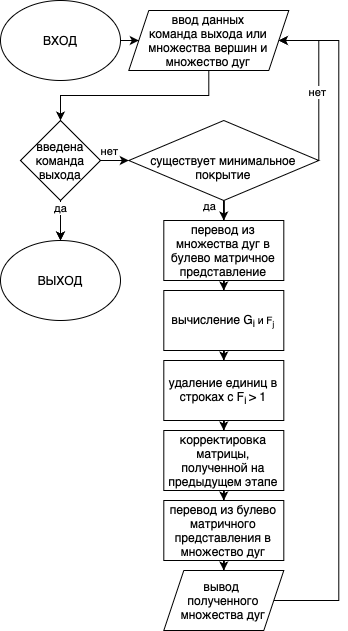
\includegraphics[width=0.7\textwidth]{diagram.png}
    \caption{Логическая блок схема алгоритма}
    \label{fig:block_diagram}
\end{figure}

\section{Оценка сложности алгоритма}

Наибольшую сложность имеет подпрограмма, исполняющая
пункт 3 алгоритма. Пункт 1 имеет сложность $O(n * m)$
Пункт 2 имеет сложность $O(n * m)$
Пункт 3 имеет сложность $O(n^2 * m^2)$, что соответсвует $4$
вложенным циклам, два из которыз проходят по строкам ($n$) и
два по столбцам ($m$).

\section{Тестовые примеры}

Пусть простой граф задан булевым матричным представлением $||M||$:

\begin{figure}[H]
    \centering
    \begin{tabular}{ c|c|c|c|c| }
              & $Y_1$ & $Y_2$ & $Y_3$ & $Y_4$ \\
        \hline
        $X_1$ & 1     & 1     & 1     & 0     \\
        \hline
        $X_2$ & 1     & 1     & 0     & 1     \\
        \hline
        $X_3$ & 0     & 0     & 1     & 0     \\
        \hline
    \end{tabular}
    \label{fig:table1}
    \caption{исходная матрица}
\end{figure}

Найдем $F_i$ и $G_i$

\begin{figure}[H]
    \centering
    \begin{tabular}{ c|c|c|c|c|c }
              & $Y_1$ & $Y_2$ & $Y_3$ & $Y_4$ & $F_i$ \\
        \hline
        $X_1$ & 1     & 1     & 1     & 0     & 3     \\
        \hline
        $X_2$ & 1     & 1     & 0     & 1     & 3     \\
        \hline
        $X_3$ & 0     & 0     & 1     & 0     & 1     \\
        \hline
        $G_j$ & 2     & 2     & 2     & 1     &
    \end{tabular}
    \label{fig:FiGj}
    \caption{$F_i$ и $G_j$}
\end{figure}

Последовательно заменим $1$ на $\circled{1}$ если $F_i > 1$ и $G_j > 1$

\begin{figure}[H]
    \centering
    \begin{tabular}{ c|c|c|c|c|c }
              & $Y_1$         & $Y_2$         & $Y_3$ & $Y_4$ & $F_i$ \\
        \hline
        $X_1$ & $\circled{1}$ & $\circled{1}$ & 1     & 0     & 1     \\
        \hline
        $X_2$ & 1             & 1             & 0     & 1     & 3     \\
        \hline
        $X_3$ & 0             & 0             & 1     & 0     & 1     \\
        \hline
        $G_j$ & 1             & 1             & 2     & 1     &
    \end{tabular}
    \label{fig:second_step_complete}
    \caption{второй этап алгоритма}
\end{figure}

Далее в $2$ строке находим $1$ - это $M_{21}$. В её
столбце отмеченная единица $\circled{1}$ - это $M_{11}$
В её строке неотмеченная единица с $G_j > 1$ - это $M_{13}$:
$G_3 = 2 > 1$. В $M_{21}$ записываем $\circled{1}$ В $M_{11}$
записываем $1$. В $M_{13}$ записываем $\circled{1}$.
$F_1$ и $G_1$ не меняются. $F_2$ и $G_3$ уменьшаются на единицу:
$F_2 = 2$ и $G_3 = 1$

\begin{figure}[H]
    \centering
    \begin{tabular}{ c|c|c|c|c|c }
              & $Y_1$         & $Y_2$         & $Y_3$         & $Y_4$ & $F_i$ \\
        \hline
        $X_1$ & 1             & $\circled{1}$ & $\circled{1}$ & 0     & 1     \\
        \hline
        $X_2$ & $\circled{1}$ & 1             & 0             & 1     & 2     \\
        \hline
        $X_3$ & 0             & 0             & 1             & 0     & 1     \\
        \hline
        $G_j$ & 1             & 1             & 1             & 1     &
    \end{tabular}
    \label{fig:third_step_complete}
    \caption{третий этап алгоритма}
\end{figure}

Далее операцию продолжить нельзя. Полученное минимальное покрытие:

\begin{figure}[H]
    \centering
    \begin{tabular}{ c|c|c|c|c| }
              & $Y_1$ & $Y_2$ & $Y_3$ & $Y_4$ \\
        \hline
        $X_1$ & 1     & 0     & 0     & 0     \\
        \hline
        $X_2$ & 0     & 1     & 0     & 1     \\
        \hline
        $X_3$ & 0     & 0     & 1     & 0     \\
        \hline
    \end{tabular}
    \label{fig:finished_coverage}
    \caption{матрица минимального покрытия}
\end{figure}

данное минимальное покрытие в виде графа можно увидеть на
Рис. \ref{fig:success_example_1}

\section{Скриншоты программы}

\begin{figure}[H]
    \centering
    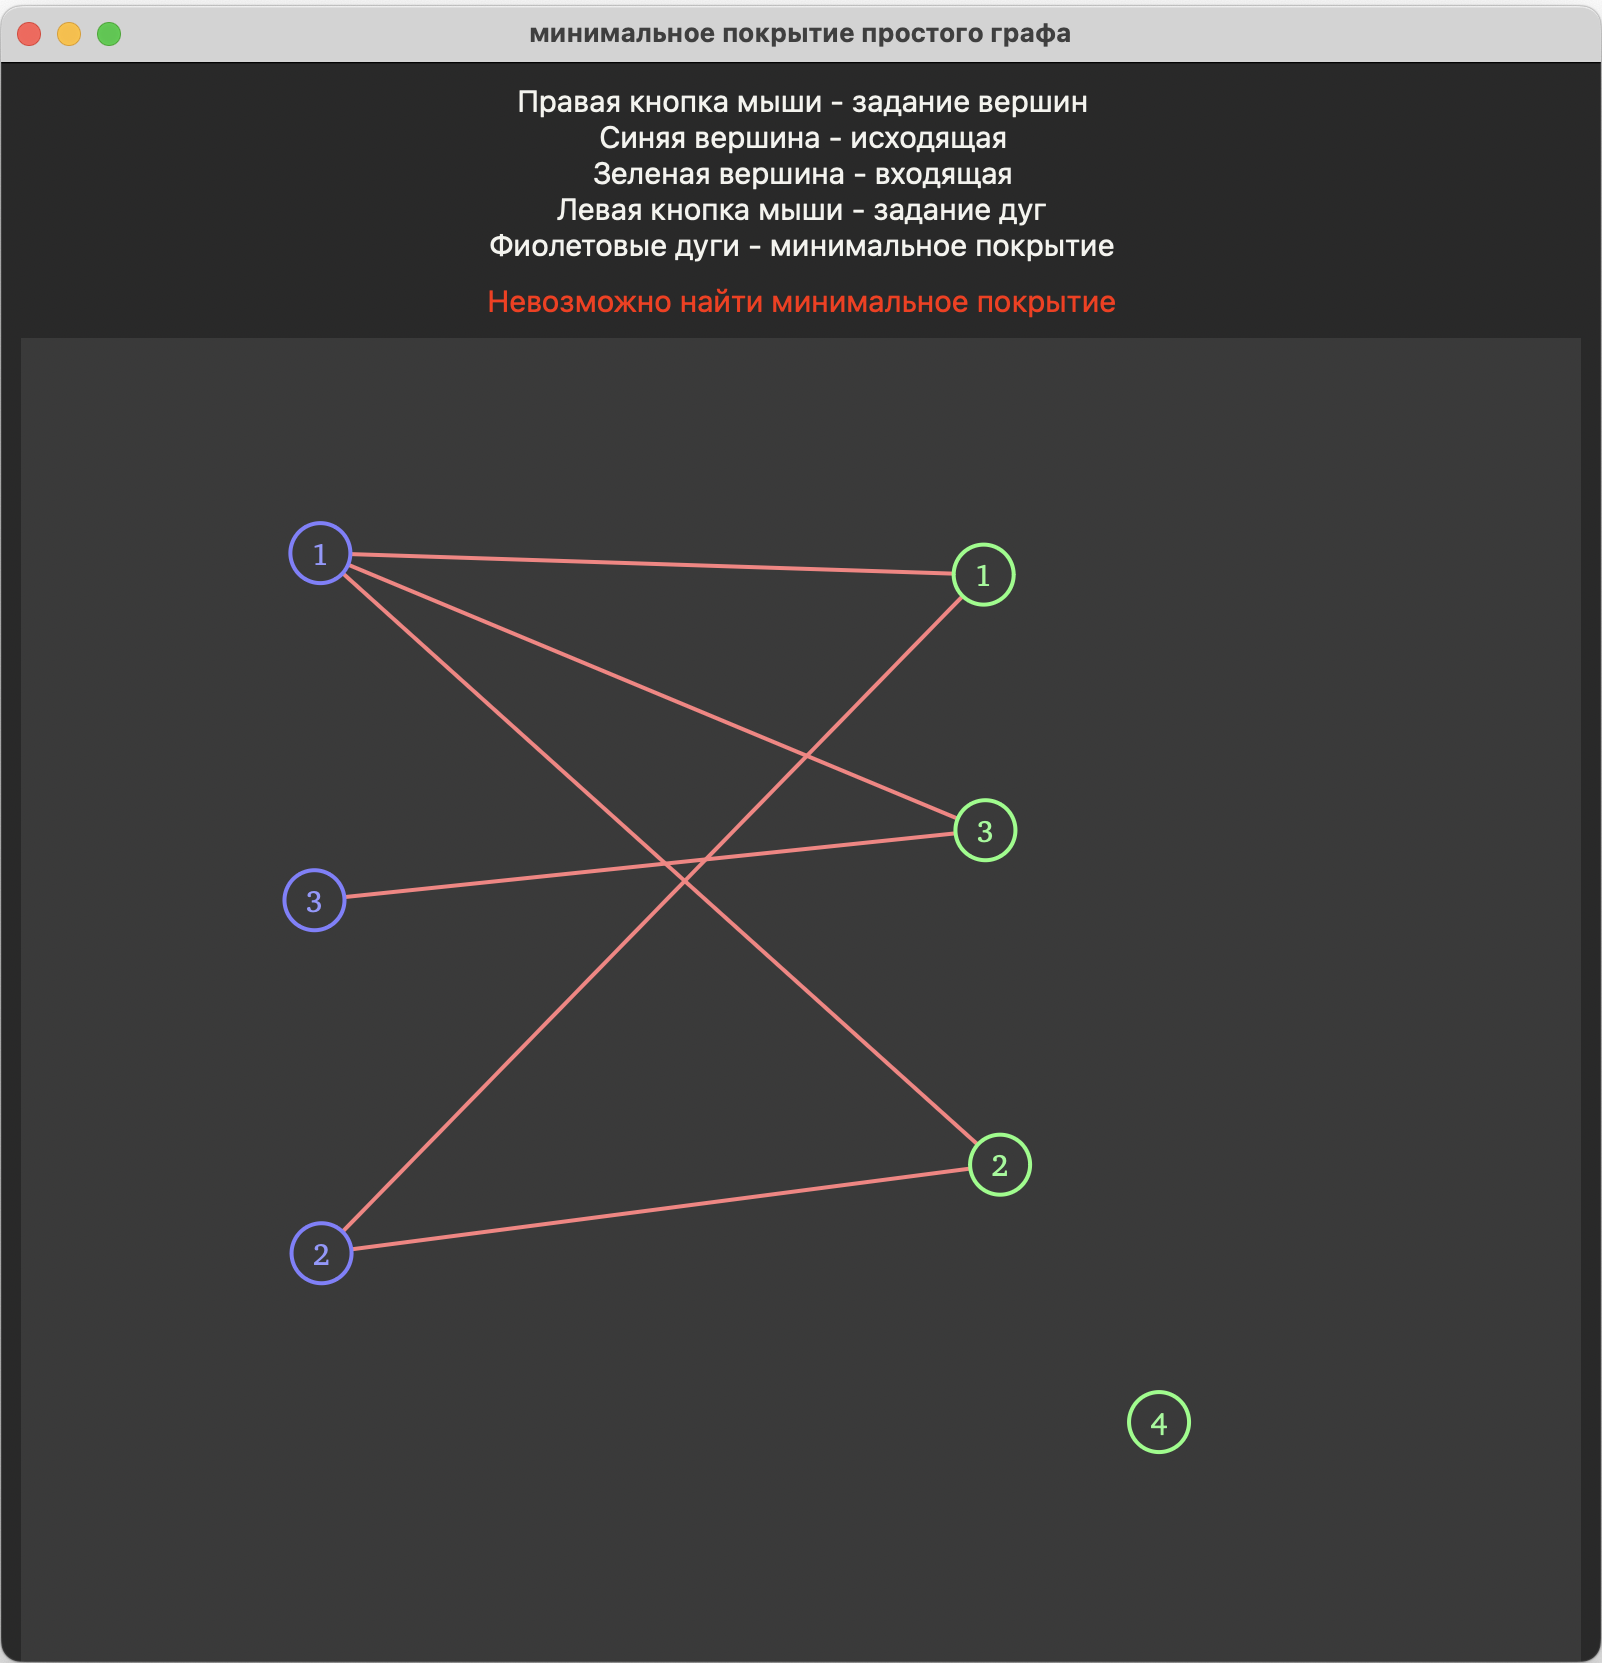
\includegraphics[width=0.5\textwidth]{screenshot1.png}
    \caption{Выдача ошибки при невозможности
        нахожения минимального покрытия}
    \label{fig:failure_example}
\end{figure}

\begin{figure}[H]
    \begin{subfigure}{0.3\textwidth}
        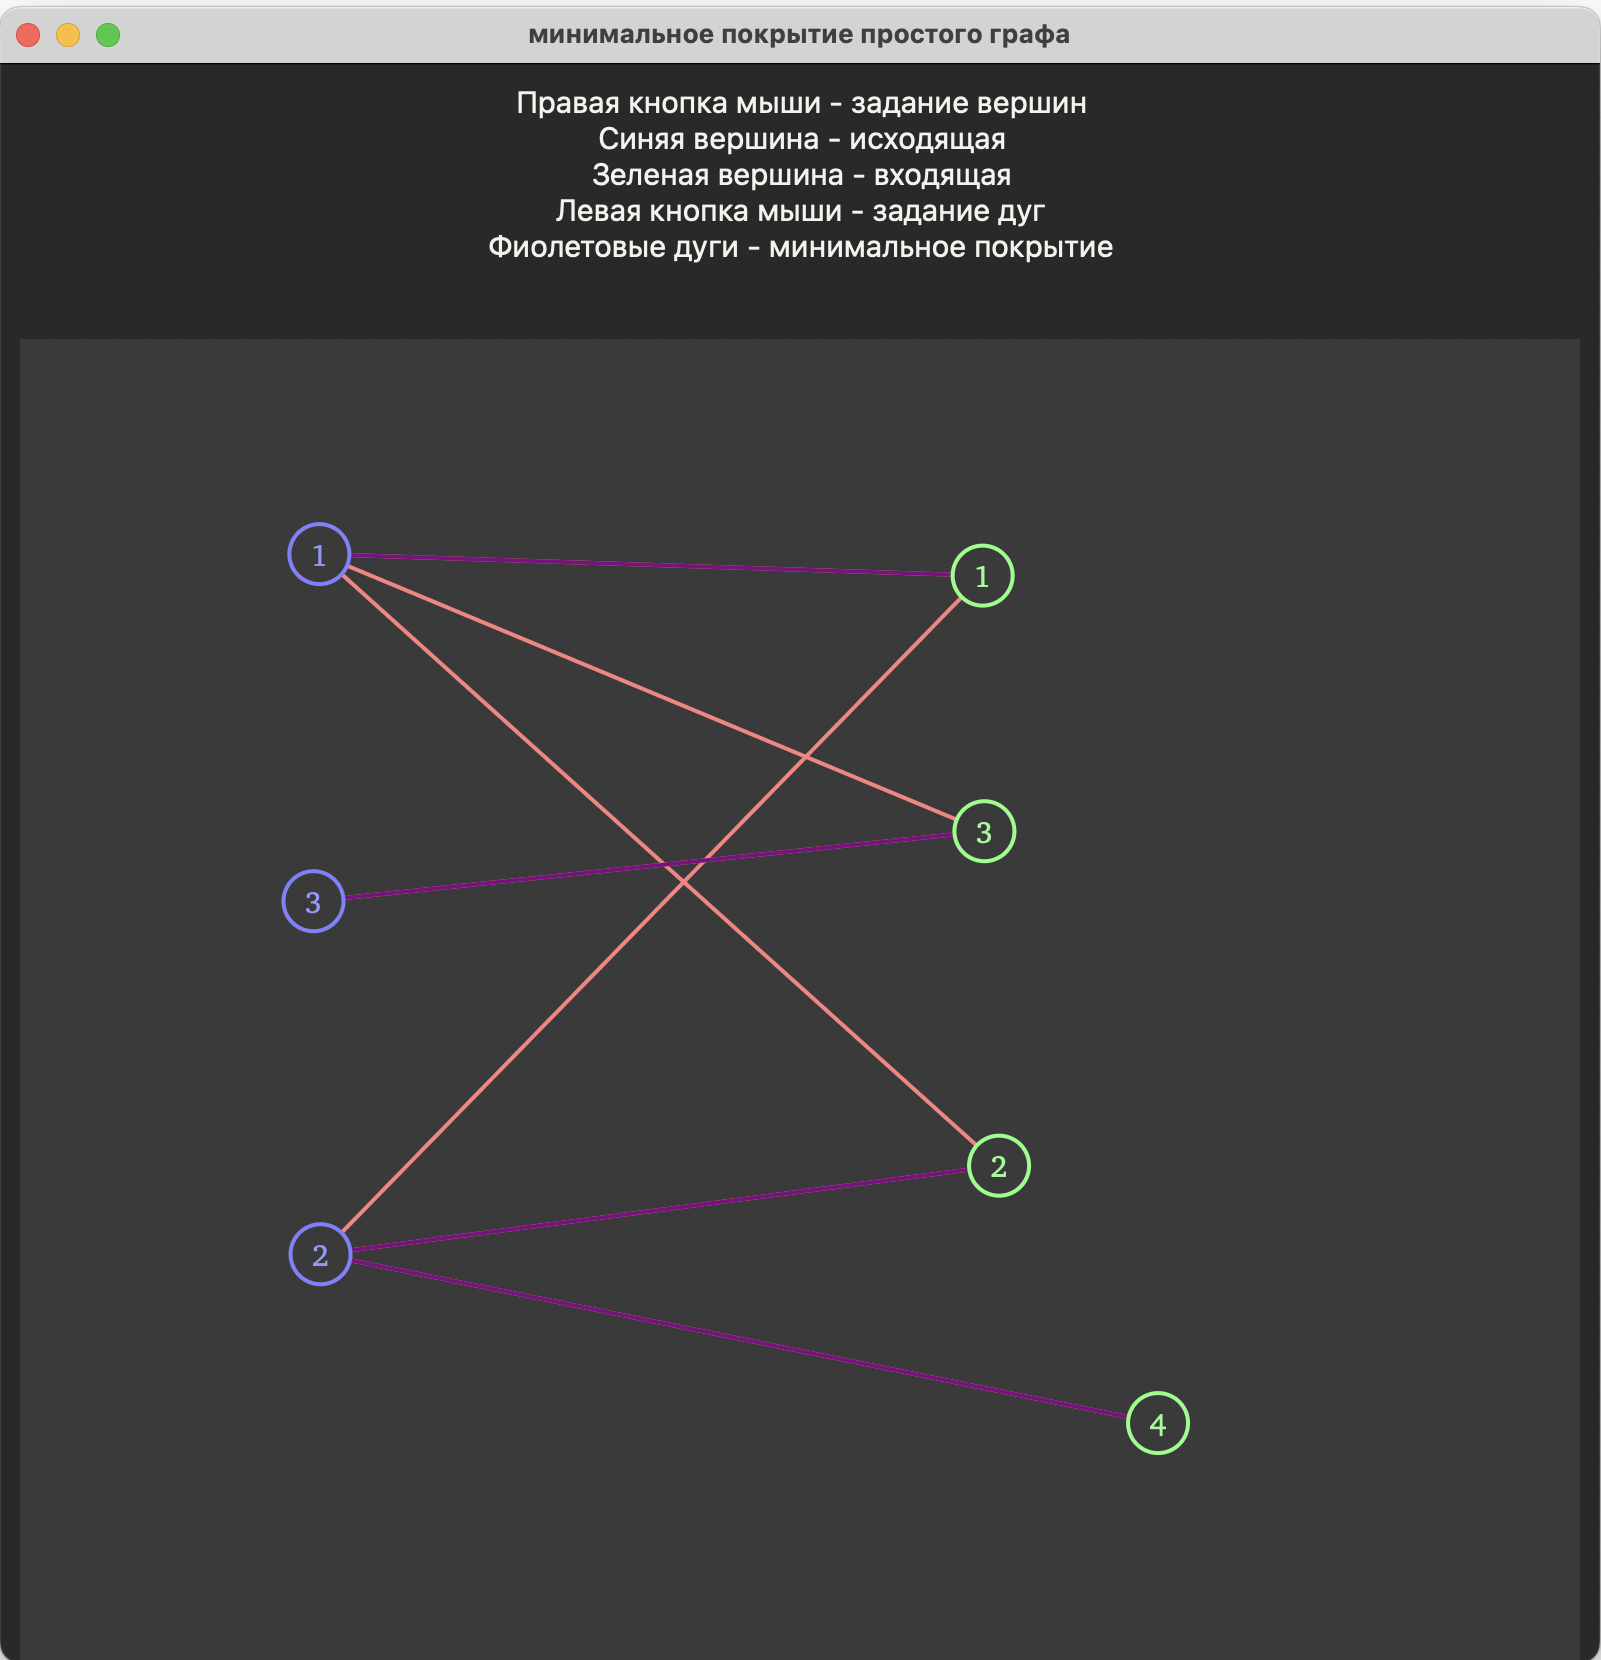
\includegraphics[width=1\textwidth]{screenshot2.png}
        \caption{Пример 1}
        \label{fig:success_example_1}
    \end{subfigure}
    \begin{subfigure}{0.3\textwidth}
        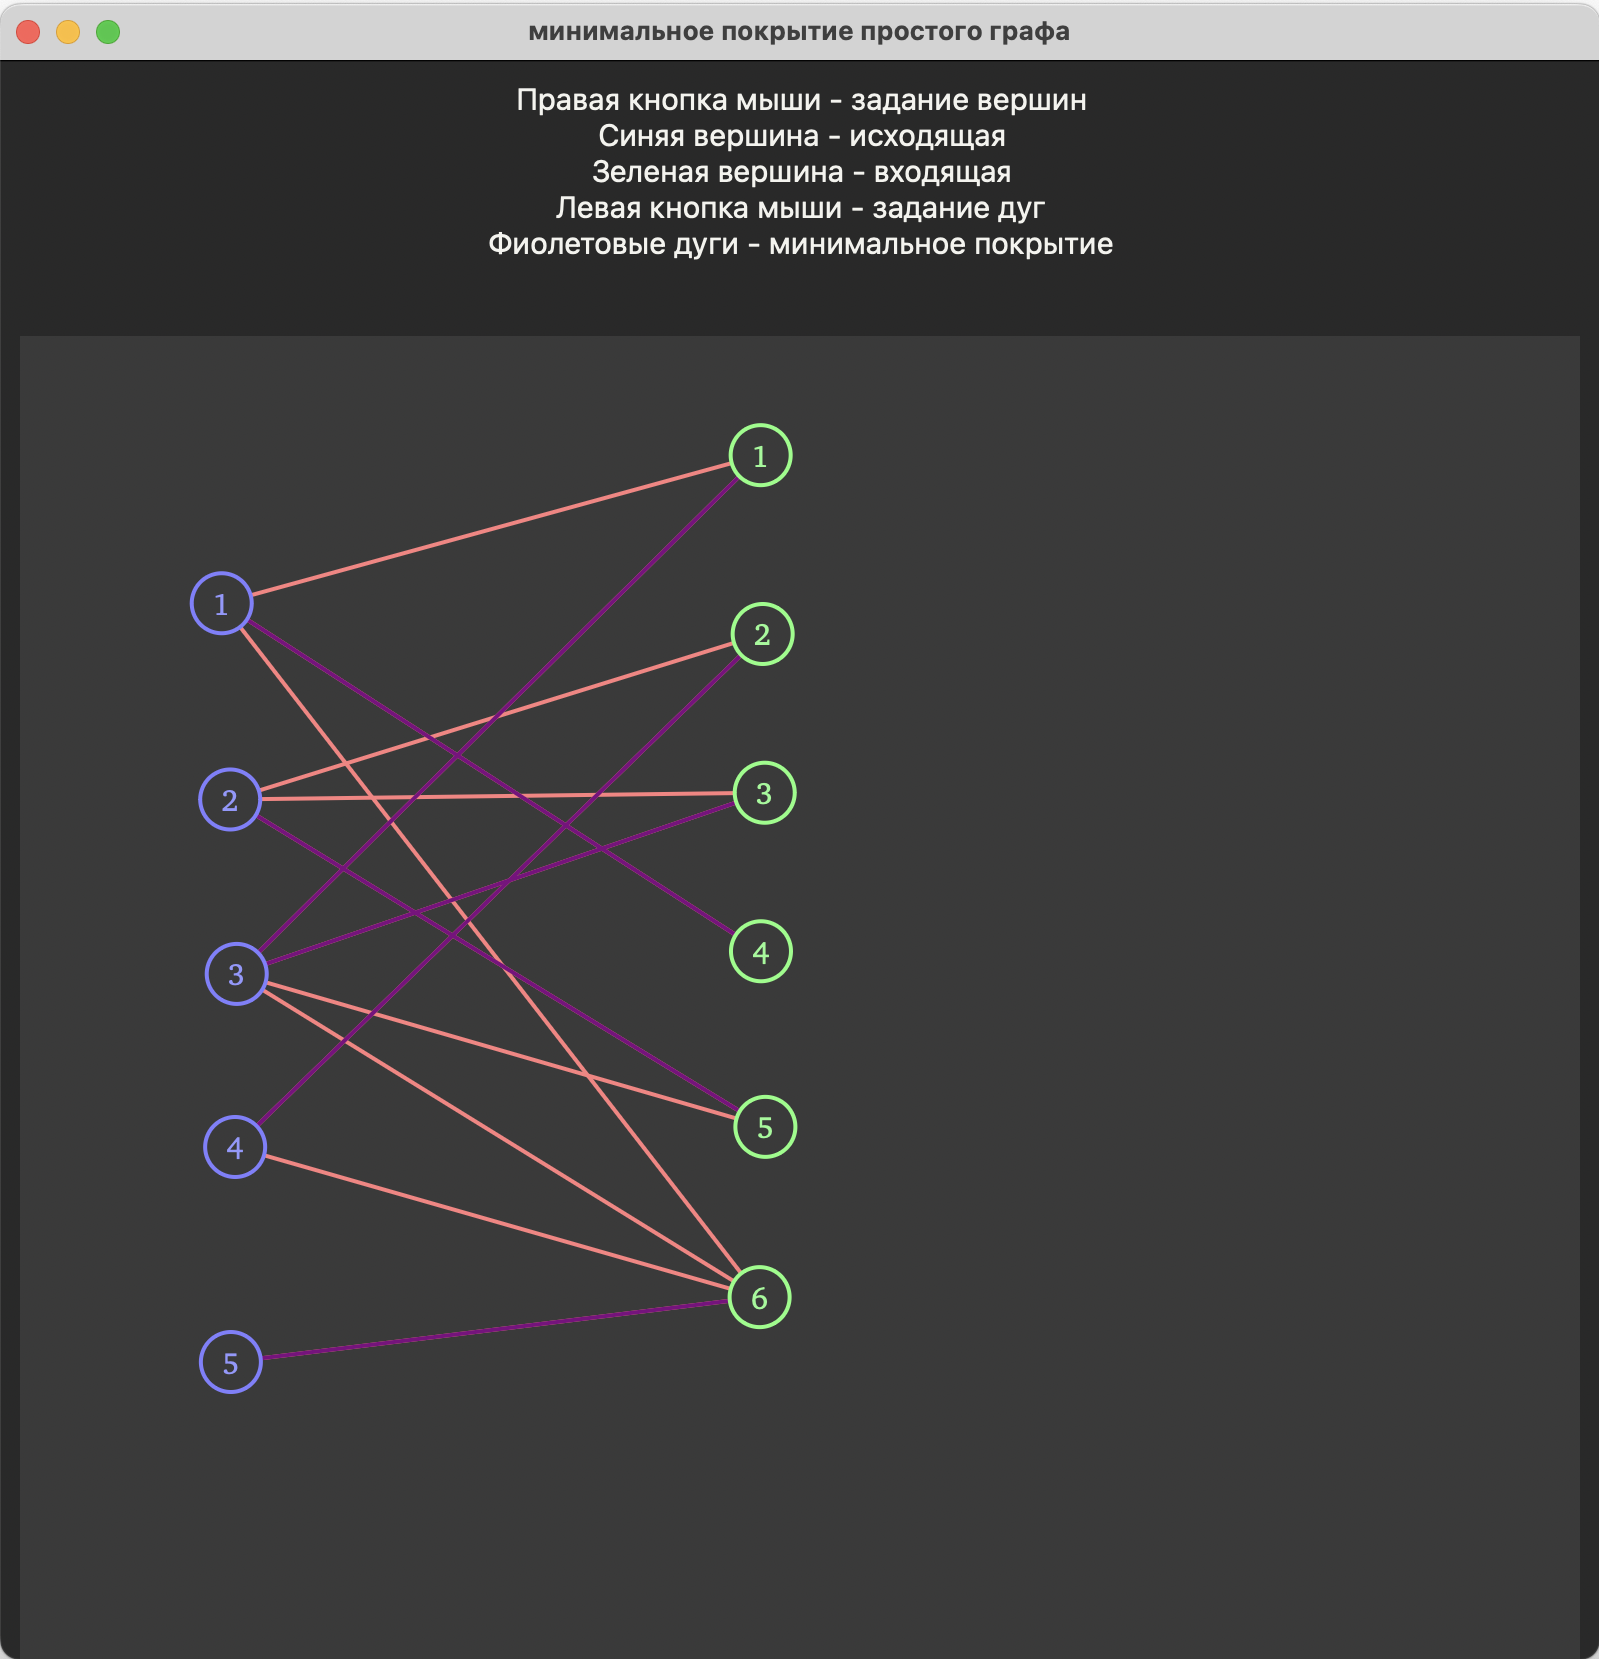
\includegraphics[width=1\textwidth]{screenshot3.png}
        \caption{Пример 2}
        \label{fig:success_example_2}
    \end{subfigure}
    \begin{subfigure}{0.3\textwidth}
        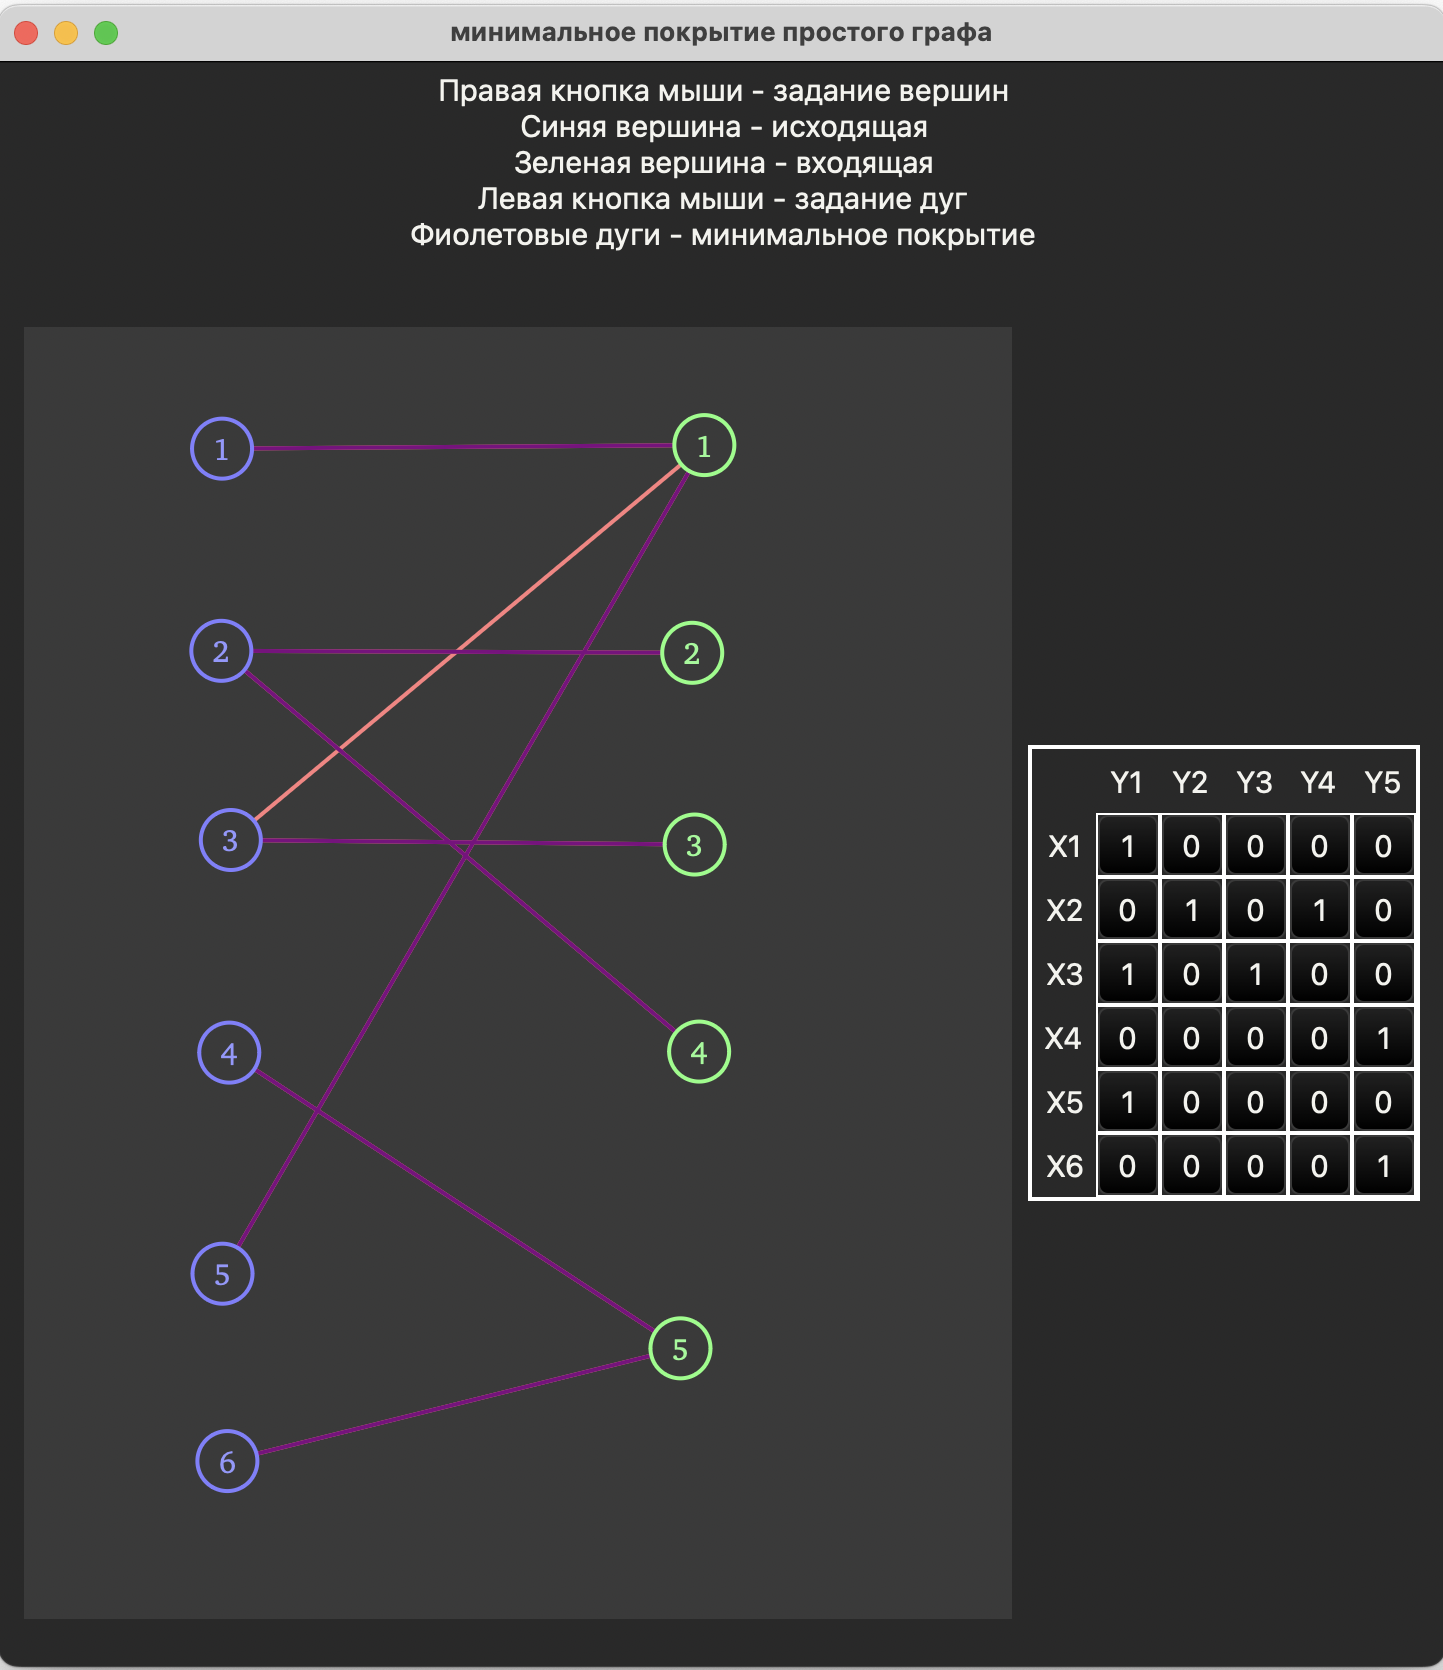
\includegraphics[width=1\textwidth]{screenshot4.png}
        \caption{Пример 3}
        \label{fig:success_example_3}
    \end{subfigure}
    \caption{Успешное нахождение минимального покрытия}
    \label{fig:success_example}
\end{figure}

\section{Пример прикладной задачи}

Простой граф используется для демонстрации связей между двумя
различными множествами. При этом не существует связей между
элементами принадлежащими одному множеству. Примером использования
данного алгоритма будет распределение студентов на мероприятия, при
условии, что каждый студент должен поучаствовать хотя бы в одном
мероприятии и на каждом мероприятии должен быть хотя бы один студент.
В данном примере первым множеством $X$ будет множество всех
студентов. Вторым множеством $Y$ будет множество всех
мероприятий.

\end{document}